\documentclass[border=6pt]{standalone}
\usepackage[T1]{fontenc}
\usepackage{amsmath}
\usepackage{tikz}
\usetikzlibrary{positioning,shadows,arrows.meta,calc}
\definecolor{dataB}{HTML}{4A86A8}\definecolor{dataF}{HTML}{E8F5FC}
\definecolor{preB}{HTML}{A0522D}\definecolor{preF}{HTML}{FDF0E4}
\definecolor{splitB}{HTML}{2E8B2E}\definecolor{splitF}{HTML}{E4FBE4}
\definecolor{regB}{HTML}{2E8B2E}\definecolor{regF}{HTML}{F0FCF0}
\definecolor{detB}{HTML}{4B0C4B}\definecolor{detF}{HTML}{F1E6F1}
\definecolor{calB}{HTML}{8B1A1A}\definecolor{calF}{HTML}{FDEEEE}
\definecolor{evB}{HTML}{4D4D4D}\definecolor{evF}{HTML}{ECECEC}
\tikzset{
 box/.style={draw, line width=1.1pt, rounded corners=5pt, align=center, inner sep=7pt,
             drop shadow={opacity=0.22, shadow xshift=1.2pt, shadow yshift=-1.2pt}},
 arr/.style={-{Latex[length=3.2mm,width=2.4mm]}, line width=1.3pt, draw=black!70},
 lin/.style={line width=1.3pt, draw=black!70},
}
\begin{document}
\large
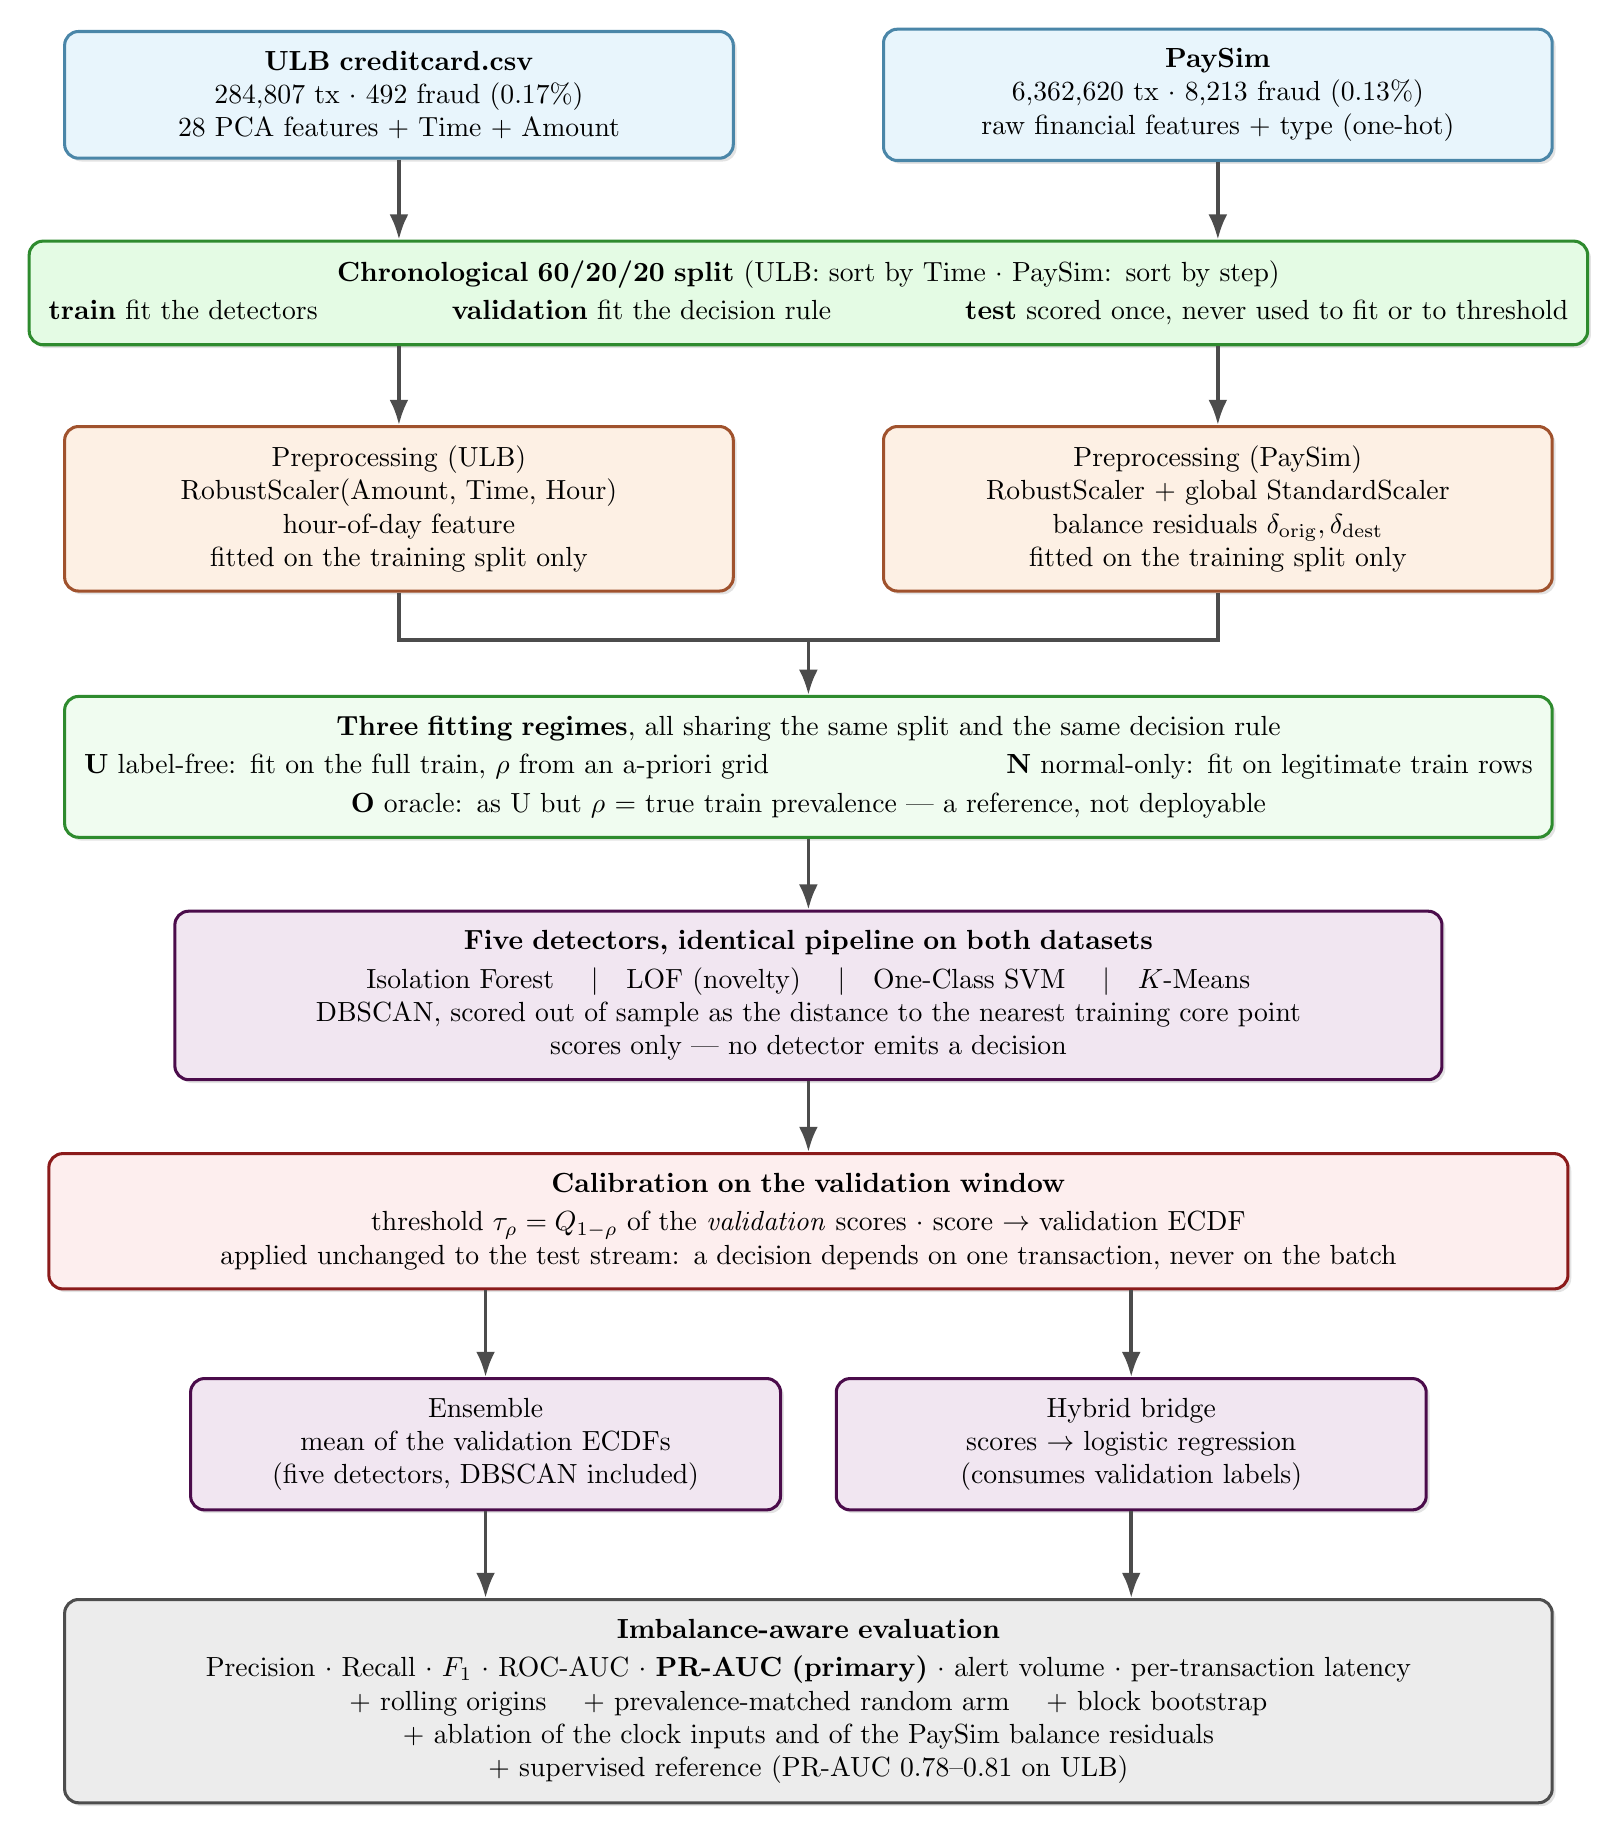
\begin{tikzpicture}[node distance=9mm]
% datasets
\node[box, draw=dataB, fill=dataF, text width=8.0cm] (ulb) at (-5.2,0)
 {\textbf{ULB creditcard.csv}\\ 284,807 tx $\cdot$ 492 fraud (0.17\%)\\ 28 PCA features + Time + Amount};
\node[box, draw=dataB, fill=dataF, text width=8.0cm] (pay) at (5.2,0)
 {\textbf{PaySim}\\ 6,362,620 tx $\cdot$ 8,213 fraud (0.13\%)\\ raw financial features + type (one-hot)};
% split
\node[box, draw=splitB, fill=splitF, text width=19.3cm, below=10mm of $(ulb.south)!0.5!(pay.south)$] (split)
 {\textbf{Chronological 60/20/20 split} (ULB: sort by Time $\cdot$ PaySim: sort by step)\\[2pt]
  \textbf{train} fit the detectors \hfill \textbf{validation} fit the decision rule \hfill \textbf{test} scored once, never used to fit or to threshold};
% preprocessing
\node[box, draw=preB, fill=preF, text width=8.0cm, below=10mm of split.south -| ulb] (pu)
 {Preprocessing (ULB)\\ RobustScaler(Amount, Time, Hour)\\ hour-of-day feature\\ fitted on the training split only};
\node[box, draw=preB, fill=preF, text width=8.0cm, below=10mm of split.south -| pay] (pp)
 {Preprocessing (PaySim)\\ RobustScaler + global StandardScaler\\ balance residuals $\delta_{\mathrm{orig}}, \delta_{\mathrm{dest}}$\\ fitted on the training split only};
% regimes
\node[box, draw=regB, fill=regF, text width=18.4cm, below=13mm of $(pu.south)!0.5!(pp.south)$] (reg)
 {\textbf{Three fitting regimes}, all sharing the same split and the same decision rule\\[2pt]
  \textbf{U} label-free: fit on the full train, $\rho$ from an a-priori grid \hfill \textbf{N} normal-only: fit on legitimate train rows\\[2pt]
  \textbf{O} oracle: as U but $\rho$ = true train prevalence --- a reference, not deployable};
% detectors
\node[box, draw=detB, fill=detF, text width=15.6cm, below=of reg] (det)
 {\textbf{Five detectors, identical pipeline on both datasets}\\[2pt]
  Isolation Forest \quad$|$\quad LOF (novelty) \quad$|$\quad One-Class SVM \quad$|$\quad $K$-Means\\
  DBSCAN, scored out of sample as the distance to the nearest training core point\\
  scores only --- no detector emits a decision};
% calibration
\node[box, draw=calB, fill=calF, text width=18.8cm, below=of det] (cal)
 {\textbf{Calibration on the validation window}\\[2pt]
  threshold \mbox{$\tau_\rho = Q_{1-\rho}$} of the \emph{validation} scores $\cdot$ score $\rightarrow$ validation ECDF\\
  applied unchanged to the test stream: a decision depends on one transaction, never on the batch};
% ensemble / hybrid
\node[box, draw=detB, fill=detF, text width=7.0cm, below=11mm of cal.south -| ulb, xshift=1.1cm] (ens)
 {Ensemble\\ mean of the validation ECDFs\\ (five detectors, DBSCAN included)};
\node[box, draw=detB, fill=detF, text width=7.0cm, below=11mm of cal.south -| pay, xshift=-1.1cm] (hyb)
 {Hybrid bridge\\ scores $\rightarrow$ logistic regression\\ (consumes validation labels)};
% evaluation
\node[box, draw=evB, fill=evF, text width=18.4cm, below=11mm of $(ens.south)!0.5!(hyb.south)$] (ev)
 {\textbf{Imbalance-aware evaluation}\\[2pt]
  Precision $\cdot$ Recall $\cdot$ $F_1$ $\cdot$ ROC-AUC $\cdot$ \textbf{PR-AUC (primary)} $\cdot$ alert volume $\cdot$ per-transaction latency\\
  + rolling origins \quad + prevalence-matched random arm \quad + block bootstrap\\
  + ablation of the clock inputs and of the PaySim balance residuals\\
  + supervised reference (PR-AUC 0.78--0.81 on ULB)};
% arrows
\draw[arr] (ulb.south) -- (ulb.south |- split.north);
\draw[arr] (pay.south) -- (pay.south |- split.north);
\draw[arr] (split.south -| pu.north) -- (pu.north);
\draw[arr] (split.south -| pp.north) -- (pp.north);
\coordinate (m) at ($(pu.south)!0.5!(pp.south) + (0,-6mm)$);
\draw[lin] (pu.south) |- (m);
\draw[lin] (pp.south) |- (m);
\draw[arr] (m) -- (reg.north);
\draw[arr] (reg.south) -- (det.north);
\draw[arr] (det.south) -- (cal.north);
\draw[arr] (cal.south -| ens.north) -- (ens.north);
\draw[arr] (cal.south -| hyb.north) -- (hyb.north);
\draw[arr] (ens.south) -- (ens.south |- ev.north);
\draw[arr] (hyb.south) -- (hyb.south |- ev.north);
\end{tikzpicture}
\end{document}
